% Options for packages loaded elsewhere
\PassOptionsToPackage{unicode}{hyperref}
\PassOptionsToPackage{hyphens}{url}
%
\documentclass[
  12pt,
]{article}
\usepackage{lmodern}
\usepackage{amssymb,amsmath}
\usepackage{ifxetex,ifluatex}
\ifnum 0\ifxetex 1\fi\ifluatex 1\fi=0 % if pdftex
  \usepackage[T1]{fontenc}
  \usepackage[utf8]{inputenc}
  \usepackage{textcomp} % provide euro and other symbols
\else % if luatex or xetex
  \usepackage{unicode-math}
  \defaultfontfeatures{Scale=MatchLowercase}
  \defaultfontfeatures[\rmfamily]{Ligatures=TeX,Scale=1}
\fi
% Use upquote if available, for straight quotes in verbatim environments
\IfFileExists{upquote.sty}{\usepackage{upquote}}{}
\IfFileExists{microtype.sty}{% use microtype if available
  \usepackage[]{microtype}
  \UseMicrotypeSet[protrusion]{basicmath} % disable protrusion for tt fonts
}{}
\makeatletter
\@ifundefined{KOMAClassName}{% if non-KOMA class
  \IfFileExists{parskip.sty}{%
    \usepackage{parskip}
  }{% else
    \setlength{\parindent}{0pt}
    \setlength{\parskip}{6pt plus 2pt minus 1pt}}
}{% if KOMA class
  \KOMAoptions{parskip=half}}
\makeatother
\usepackage{xcolor}
\IfFileExists{xurl.sty}{\usepackage{xurl}}{} % add URL line breaks if available
\IfFileExists{bookmark.sty}{\usepackage{bookmark}}{\usepackage{hyperref}}
\hypersetup{
  pdftitle={Hurricane Michael and Floridian Turnout},
  pdfauthor={Kevin Morris},
  hidelinks,
  pdfcreator={LaTeX via pandoc}}
\urlstyle{same} % disable monospaced font for URLs
\usepackage[margin=1in]{geometry}
\usepackage{longtable,booktabs}
% Correct order of tables after \paragraph or \subparagraph
\usepackage{etoolbox}
\makeatletter
\patchcmd\longtable{\par}{\if@noskipsec\mbox{}\fi\par}{}{}
\makeatother
% Allow footnotes in longtable head/foot
\IfFileExists{footnotehyper.sty}{\usepackage{footnotehyper}}{\usepackage{footnote}}
\makesavenoteenv{longtable}
\usepackage{graphicx}
\makeatletter
\def\maxwidth{\ifdim\Gin@nat@width>\linewidth\linewidth\else\Gin@nat@width\fi}
\def\maxheight{\ifdim\Gin@nat@height>\textheight\textheight\else\Gin@nat@height\fi}
\makeatother
% Scale images if necessary, so that they will not overflow the page
% margins by default, and it is still possible to overwrite the defaults
% using explicit options in \includegraphics[width, height, ...]{}
\setkeys{Gin}{width=\maxwidth,height=\maxheight,keepaspectratio}
% Set default figure placement to htbp
\makeatletter
\def\fps@figure{htbp}
\makeatother
\setlength{\emergencystretch}{3em} % prevent overfull lines
\providecommand{\tightlist}{%
  \setlength{\itemsep}{0pt}\setlength{\parskip}{0pt}}
\setcounter{secnumdepth}{5}
\usepackage{rotating}
\usepackage{setspace}\doublespacing
\newcommand{\beginsupplement}{\setcounter{table}{0}  \renewcommand{\thetable}{A\arabic{table}} \setcounter{figure}{0} \renewcommand{\thefigure}{A\arabic{figure}}}
\usepackage{booktabs}
\usepackage{longtable}
\usepackage{array}
\usepackage{multirow}
\usepackage{wrapfig}
\usepackage{float}
\usepackage{colortbl}
\usepackage{pdflscape}
\usepackage{tabu}
\usepackage{threeparttable}
\usepackage{threeparttablex}
\usepackage[normalem]{ulem}
\usepackage{makecell}
\usepackage{xcolor}

\title{Hurricane Michael and Floridian Turnout\thanks{The author thanks Many People for their comments on this project. All errors are my responsibility.}}
\author{Kevin Morris\footnote{Researcher, Brennan Center for Justice at NYU School of Law, 120 Broadway Ste 1750, New York, NY 10271 (\href{mailto:kevin.morris@nyu.edu}{\nolinkurl{kevin.morris@nyu.edu}})}}
\date{February 25, 2020}

\begin{document}
\maketitle
\begin{abstract}
This is an abstract.
\end{abstract}

\pagenumbering{gobble}
\pagebreak

\pagenumbering{arabic}

\hypertarget{research-design-and-expectations}{%
\section*{Research Design and Expectations}\label{research-design-and-expectations}}
\addcontentsline{toc}{section}{Research Design and Expectations}

Voters who lived in counties covered by the executive order were ``treated'' in multiple ways. To begin with, they faced terrible weather. Homes were destroyed and some community members were killed by the storm, likely depressing individuals' propensity to vote. In addition to the weather, however, voters were treated by the responses of the counties in which they lived. Counties may have shifted funds away from GOTV efforts, for instance, to repairing damaged polling places\footnote{Data received from public records requests filed with the treated counties leaves us unable to determine whether this did in fact occur. It is, nonetheless, possible.} --- this too could have reduced turnout. Finally, they were treated by the executive order. The executive order may have increased turnout to levels higher than it would have been with just the effects of the storm and county-level responses.

We begin by testing the net effect of each of these treatments on individual-level turnout. Our central identification strategy involves the use of difference-in-differences models. By comparing historical and 2018 turnout for voters in the counties hit by the storm to historical and 2018 turnout of voters elsewhere in the state, we can estimate the effect of the storm on turnout. To ensure a high-quality difference-in-differences specification, we do not include all untreated voters in our control group; rather, we match each treated voter with five untreated voters along a battery of individual- and neighborhood-level characteristics. Untreated voters who do not serve as matches are excluded from our models. Although it may seem counterintuitive to exclude data from our models, this matching procedure substantially improves the parallel trends assumptions necessary for a rigorous difference-in-differences analysis.

This design allows us to test our first hypothesis:

\textbf{Hypothesis 1:} Turnout in the eight treated counties was lower in 2018 due to the combined effects of the hurricane, county-level responses, and the executive order.

The above research design does not allow us to disentangle the effects of the storm from the effects of election administration in response to the storm. In order to control for the effects of the storm, we construct a second set of difference-in-differences models leveraging a much smaller pool of voters. We begin by identifying all voters who lived in a voter precinct in a county that bordered a voter precint in a different, untreated county. We then match each voter in the treated precinct to a voter in her neighboring precinct in the untreated county. Because each pair of voters lived in close geographic proximity to one another, we assume that each paired set of voters faced the same weather conditions in the 2018 election. Any observed turnout differential, therefore, can be attributed to differences in election administration. This allows us to test our second hypothesis:

\textbf{Hypothesis 2:} After controlling for weather, we expect that turnout in the treated counties was higher than in neighboring, untreated counties. Treated and control voters all faced similar weather in the 2018 election, but voters in the treated counties had election administrators that could more flexibly respond to the adverse weather conditions. We hypothesize that this increased flexibility was successful at boosting turnout.

After identifying the high-level turnout effects of Hurricane Michael in 2018, we examine how the storm altered the vote method of participants.

\textbf{Hypothesis 3:} Because the executive order specifically lifted restrictions on early and absentee voting, we expect that the executive order increased the share of participants who voted early or cast an absentee ballot in the 2018 election.

\hypertarget{results}{%
\section*{Results}\label{results}}
\addcontentsline{toc}{section}{Results}

We begin by matching each registered voter in the eight treated counties to five untreated voters elsewhere in the state using a genetic matching algorithm.\footnote{Due to computing constraints, the matching weights were constructed using a five percent random sample stratified by treatment status.} The individual-level characteristics come directly from the registered voter file. The two neighborhood-level characteristics included --- median income and share of the population with some collegiate education --- are estimated at the block group level, and come from the ACS 5-year estimates ending with 2018.

Table \ref{tab:full-bal} demonstrates the results of this matching procedure. As Table \ref{tab:full-bal} makes clear, voters in the affected counties were considerably more likely to be white and identify as Republicans, and live in lower-income neighborhoods, than voters in the rest of the state. The post-match control group, however, looks substantially similar to the treated voters.

\begin{singlespace}
\begin{table}[H]

\caption{\label{tab:balance-tab-full}\label{tab:full-bal} Balance Table for Statewide Matching}
\centering
\resizebox{\linewidth}{!}{
\begin{tabular}[t]{lllllrrrr}
\toprule
\multicolumn{1}{c}{ } & \multicolumn{2}{c}{Means: Unmatched Data} & \multicolumn{2}{c}{Means: Matched Data} & \multicolumn{4}{c}{Percent Improvement} \\
\cmidrule(l{3pt}r{3pt}){2-3} \cmidrule(l{3pt}r{3pt}){4-5} \cmidrule(l{3pt}r{3pt}){6-9}
 & Treated & Control & Treated & Control & Mean Diff & eQQ Med & eQQ Mean & eQQ Max\\
\midrule
\%White & 76.0\% & 63.0\% & 76.0\% & 76.0\% & 99.34 & 100.00 & 100.00 & 100.00\\
\% Black & 17.0\% & 13.0\% & 17.0\% & 17.0\% & 98.82 & 100.00 & 100.00 & 100.00\\
\% Latino & 2.0\% & 17.0\% & 2.0\% & 2.0\% & 99.87 & 100.00 & 100.00 & 100.00\\
\% Asian & 1.0\% & 2.0\% & 1.0\% & 1.0\% & 97.39 & 100.00 & 100.00 & 100.00\\
\% Female & 52.0\% & 52.0\% & 52.0\% & 52.0\% & 85.72 & 100.00 & 100.00 & 100.00\\
\% Male & 47.0\% & 45.0\% & 47.0\% & 47.0\% & 96.85 & 100.00 & 100.00 & 100.00\\
Age & 52.23 & 52.35 & 52.23 & 52.29 & 51.12 & 84.71 & 83.16 & 78.10\\
\% Democrat & 39.0\% & 37.0\% & 39.0\% & 39.0\% & 90.29 & 100.00 & 100.00 & 100.00\\
\% Republican & 43.0\% & 35.0\% & 43.0\% & 44.0\% & 95.08 & 99.84 & 99.84 & 99.84\\
\% with Some College & 69.0\% & 75.0\% & 69.0\% & 69.0\% & 97.78 & 98.83 & 98.08 & 90.60\\
Median Income & \$50,612 & \$62,921 & \$50,612 & \$50,796 & 98.51 & 97.16 & 95.42 & 88.79\\
\bottomrule
\end{tabular}}
\end{table}
\end{singlespace}

After matching the individual voters, we can construct historical turnout estimates for the treated and control voters. Figure \ref{fig:full-to} plots the turnout in the past few elections for our treated and control voters. As Figure \ref{fig:full-to} makes clear, the gap between treated and control groups was constant from 2010 -- 2016. In 2018 however --- the year when Hurricane Michael wreaked havoc on voters in the treatment group --- the gap widens substantially. Although turnout among all voters was higher in 2018 than in 2014, turnout rose by substantially less for the treated voters.

\begin{figure}[H]

{\centering 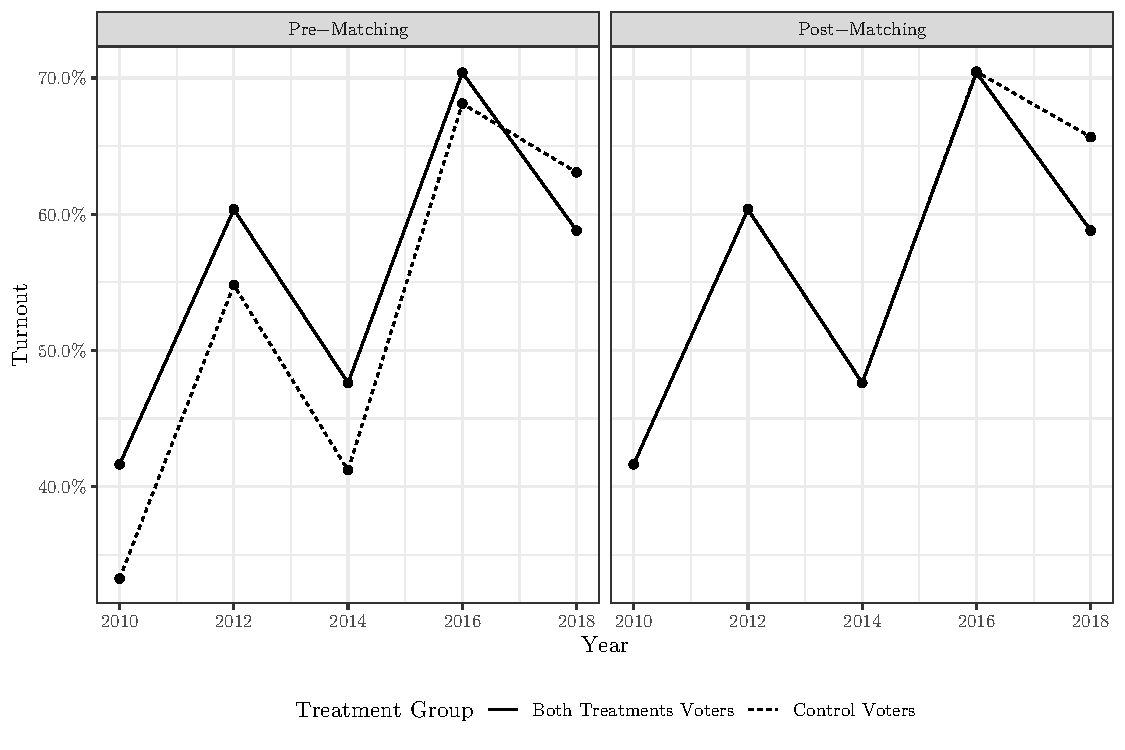
\includegraphics{hurricane_michael_files/figure-latex/full-to-chunk-1} 

}

\caption{\label{fig:full-to}General Election Turnout for Treated and Control Voters, 2010 -- 2018}\label{fig:full-to-chunk}
\end{figure}

Table \ref{tab:full-dind} formalizes Figure \ref{fig:full-to} into a differences-in-differences regression specification. I employ a logistic model, as the dependent variable --- turnout --- is binary. The dependent variable takes the value 1 if a voter cast a ballot in a given year, and 0 if she did not. Model 1 includes only three variables in addition to the constant. \emph{D(Treated)} measures the gap between treated and control voters in the 2010 -- 2016 period. \emph{D(2018)} measures the increase in turnout observed among control voters in 2018, while \emph{D(Treated) × D(2018)} measures whether turnout in 2018 departed further or less from the baseline for the treated voters than the control voters. Model 2 includes the same variables, but also includes the characteristics on which the voters were matched. Model 3, finally, also includes measures for congressional district competitiveness. Because this variable is ``downstream'' of treatment --- that is to say, the effect of the hurricane could have impacted the competitiveness of certain races --- it is not included in the first two models. It should be noted that each of the treated voters lived in uncontested congressional districts. Robust standard errors are clustered at the level of the match.

\begin{singlespace}

\input{"../temp/dind_full.tex"}
\end{singlespace}

Exponentiating the coefficients in Table \ref{tab:full-dind} indicates that Hurricane Michael, net of any county- and state-level responses, reduced turnout by between 28.3 and 32.3 percentage points.

There was substantial differences in the depressed turnout in the different counties. Turnout in Bay, Calhoun, and Jackson Counties, for instance, was between 60 and 70 percent of what it would have been absent the hurricane; counterintuitively, the treatment effect in Franklin County is associated with a 20 to 23 percentage point increase in turnout. Figure \ref{fig:county-effects} plots the treatment effect for each county.

\begin{figure}[H]

{\centering 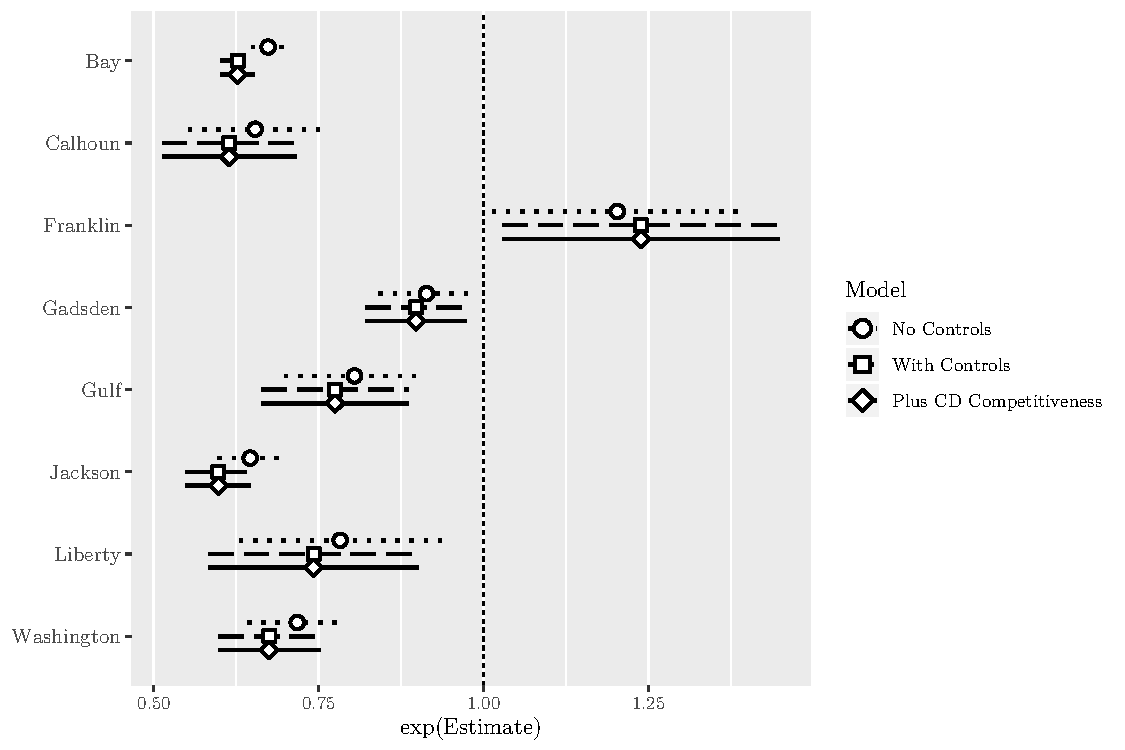
\includegraphics{hurricane_michael_files/figure-latex/county-effect-chunk-1} 

}

\caption{\label{fig:county-effects}Treatment Effect by Treated County}\label{fig:county-effect-chunk}
\end{figure}

\hypertarget{turnout-in-the-panhandle}{%
\section*{Turnout in the Panhandle}\label{turnout-in-the-panhandle}}
\addcontentsline{toc}{section}{Turnout in the Panhandle}

Hypothesis: Although turnout was depressed in the treated counties, it was higher than it would have been absent the executive order.

In this study, we are interested in understanding not only the effect the hurricane had on turnout, but also the efficacy of the executive order. Disentangling the effect of the hurricane from the effect of the executive order requires a different analytical strategy.

To test the efficacy of the executive order, we leverage the somewhat random borders of the treated counties. There is little reason to believe that the effects of a hurricane would change dramatically along county borders. We assume, therefore, that voters who lived nearby one another, but on either side of a county border, faced the same weather issues during the 2018 election. Any difference in turnout observed between the group that lived just over a county border from one another, therefore, can be attributed to the executive order (or the counties' responses to it). We expect turnout in the treated counties to be higher than in untreated counties, because the treatment should theoretically reduce the cost of voting in those counties.

We begin by identifying all voter precincts in ``treated'' counties that border voter precincts in ``untreated'' counties. Figure \ref{fig:map} shows the border precincts in treated and untreated counties, as well as the precincts that do not fall along the border of a county with a different treatment status. Border precincts in treated counties are in the darkest shade of gray; border precincts in untreated counties are slightly lighter; the precincts that are not used for this analysis are in the lightest shade. Precinct borders are drawn in white, while county borders are drawn in black. Because Gulf and Calhoun Counties are entirely surrounded by other treated counties, no precincts from these counties are used in this analysis.

\begin{figure}[H]

{\centering 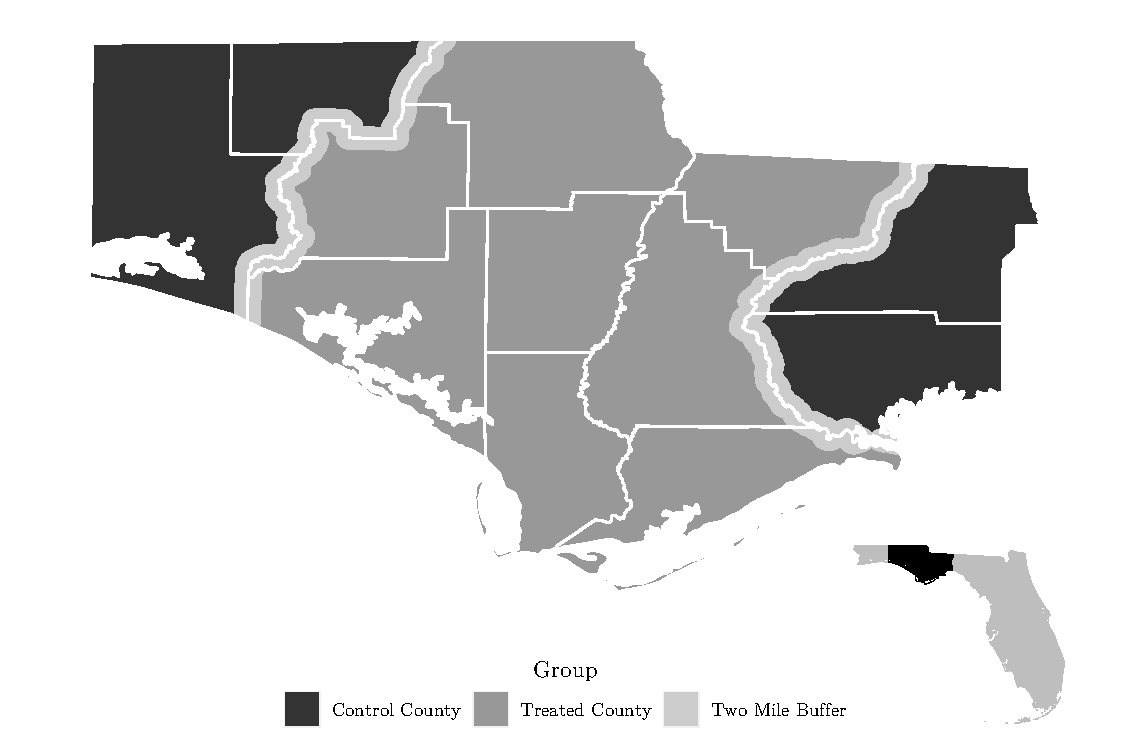
\includegraphics{hurricane_michael_files/figure-latex/map-chunk-1} 

}

\caption{\label{fig:map}Treated, Control, and Discarded Precincts in the Treated Region}\label{fig:map-chunk}
\end{figure}

Each voter in a treated, border precinct is matched with one voter in a neighboring precinct in an untreated county. In some cases, precincts on either side of the border are in different congressional districts. This would pose a problem if these races were contested, but every precinct included was located entirely in an uncontested congressional district.\footnote{One precinct pair, however, is excluded: the Liberty County 5th Precinct was located in a congressional district that went uncontested by Democrats, but borders Precinct 2365 in Leon County, located in a district uncontested by a Republican. All other cross-county precinct pairs faced the same congressional race landscape.} As before, we match on individual- and neighborhood-level characteristics. Table \ref{tab:balance-ll} presents the results of this matching exercise.

\begin{singlespace}
\begin{table}[H]

\caption{\label{tab:balance-tab-ll}\label{tab:balance-ll} Balance Table for Border Precinct Matching}
\centering
\resizebox{\linewidth}{!}{
\begin{tabular}[t]{lllllrrrr}
\toprule
\multicolumn{1}{c}{ } & \multicolumn{2}{c}{Means: Unmatched Data} & \multicolumn{2}{c}{Means: Matched Data} & \multicolumn{4}{c}{Percent Improvement} \\
\cmidrule(l{3pt}r{3pt}){2-3} \cmidrule(l{3pt}r{3pt}){4-5} \cmidrule(l{3pt}r{3pt}){6-9}
 & Treated & Control & Treated & Control & Mean Diff & eQQ Med & eQQ Mean & eQQ Max\\
\midrule
\%White & 75.0\% & 83.0\% & 75.0\% & 75.0\% & 99.91 & 99.93 & 99.93 & 99.93\\
\% Black & 21.0\% & 12.0\% & 21.0\% & 21.0\% & 99.31 & 99.30 & 99.30 & 99.30\\
\% Latino & 2.0\% & 2.0\% & 2.0\% & 2.0\% & 99.88 & 100.00 & 100.00 & 100.00\\
\% Asian & 0.0\% & 1.0\% & 0.0\% & 0.0\% & 93.07 & 93.05 & 93.05 & 93.05\\
\% Female & 53.0\% & 53.0\% & 53.0\% & 53.0\% & 94.65 & 95.16 & 95.16 & 95.16\\
\% Male & 45.0\% & 46.0\% & 45.0\% & 45.0\% & 90.01 & 89.01 & 89.01 & 89.01\\
Age & 52.54 & 51.61 & 52.54 & 52.52 & 98.34 & 67.87 & 60.84 & 43.35\\
\% Democrat & 44.0\% & 39.0\% & 44.0\% & 44.0\% & 99.84 & 99.90 & 99.90 & 99.90\\
\% Republican & 42.0\% & 45.0\% & 42.0\% & 42.0\% & 98.65 & 98.58 & 98.58 & 98.58\\
\% with Some College & 64.0\% & 67.0\% & 64.0\% & 67.0\% & -27.23 & -3.90 & -21.66 & -29.52\\
Median Income & \$47,598 & \$49,407 & \$47,598 & \$50,132 & -40.13 & 20.49 & 8.70 & 1.05\\
\bottomrule
\end{tabular}}
\end{table}
\end{singlespace}

Although the matching exercise does not improve the neighborhood-level characteristics, each of the individual-level characteristics are much improved. The lack of balance on the neighborhood-level characteristics does not appear to cause us to violate the parallel trends assumption; as Figure \ref{fig:ll-to} makes clear, the gap between treated and control voters in the 2010 -- 2016 period remains constant.

\begin{figure}[H]

{\centering 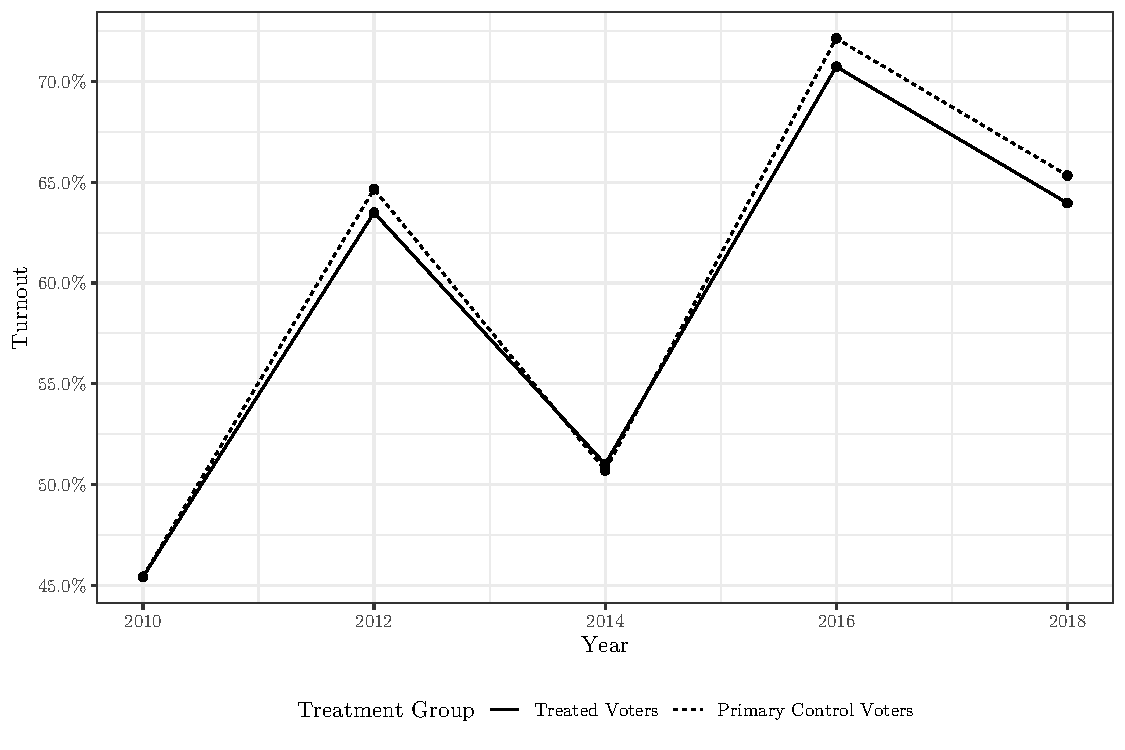
\includegraphics{hurricane_michael_files/figure-latex/ll-to-chunk-1} 

}

\caption{\label{fig:ll-to}General Election Turnout for Border Precinct Matches, 2010 -- 2018}\label{fig:ll-to-chunk}
\end{figure}

The trends in Figure \ref{fig:ll-to} are surprising: although turnout for voters in the treated group was generally higher in the 2010 -- 2016 period, the difference disappeared in 2018. The control voters, in fact, turned out at higher rates in 2018 than the control voters. This implies that, even though these voters generally saw the same weather in 2018, turnout was markedly depressed in the places where the executive order should have made it \emph{easier} to vote. Table \ref{tab:dind-ll} formalizes Figure \ref{fig:ll-to} into a logistic regression. Model 1 includes only the difference-in-difference dummies, while Model 2 adds in the characteristics on which the matching was performed. In both models, robust standard errors are clustered at the level of the match.

\begin{singlespace}

\input{"../temp/dind_ll.tex"}
\end{singlespace}

As Figure \ref{fig:ll-to} makes clear visually, the treatment effect is substantial. Exponentiating the coefficients in Models 1 and 2 in Table \ref{tab:dind-ll} indicates that turnout in 2018 among voters who lived in treated counties was between 87 and 85 percent (respectively) as high as it would have been absent the treatment.

\end{document}
